%!TEX root = ../copatterns-thesis.tex
\chapter{Idris}
\label{cha:idris}
Idris is a general-purpose functional programming language with full dependent
types. Having full dependent types means that the type and the term level
language is one and the same, such that types \emph{are} in fact terms, making
computations on types as easily definable as computations on other kinds of
terms. Idris has native support for dependent product and sum types,
(co)inductive families, and dependent pattern matching. Additionally, Idris
allows the definition of provably total functions, which is imperative when
exploiting the principle of programs-as-proofs to ensure program correctness. 

In order to show which parts of the language implementation must be manipulated
when implementing copatterns and inference of guarded recursion, respectively, this chapter
discusses the internal structure of the Idris compiler. Providing a
comprehensive description of the compiler is not within the scope of this
presentation, but many of the details not covered
here have been described thoroughly by Brady\,\citep{BradyIdrisImpl13}.

% To understand how an implementation of guarded recursion could be realized in Idris, we must first understand the internal structure of the language. In this section we will first outline the overall structure of Idris and then dig into specific parts relevant to guarded recursion. This is not a thorough description of all of Idris's components, but rather an explanation of parts of the language. For more reading on this topic see Edwin Brady's .%todo: REF
\section{Overview}
%Idris -> Idris- -> TT -> Executable
\begin{figure}
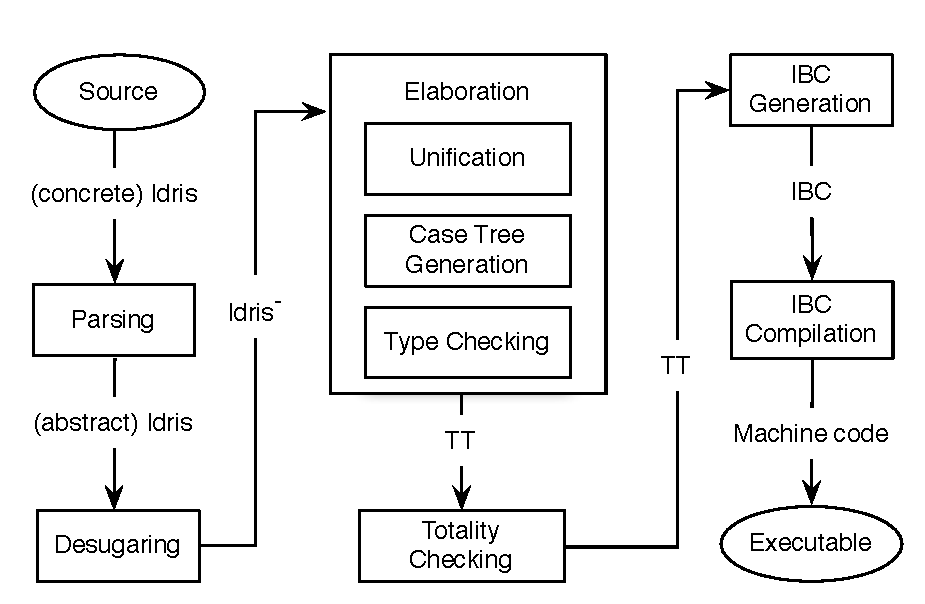
\includegraphics[scale=0.9]{figures/Idris-overview}
\caption{The phases of the Idris compiler. Phases are shown as rectangles, and
  each transition (arrow) is annotated with the input or output representation
  of a given phase. Ovals designate endpoints.}
\label{fig:idris-overview}
\end{figure}
An overview of the different phases of the Idris compiler is shown in
Figure~\ref{fig:idris-overview}. Starting with concrete Idris source code and
ending with a binary executable, each rectangle represents one phase of
compilation. During compilation, the input program is represented in several
different internal languages. Each arrow in Figure~\ref{fig:idris-overview}
is ascribed with the language in which the input program is represented when entering
or leaving a phase, respectively. Omitting a description of the machine code, these are:
\begin{itemize}
\item \textbf{(concrete) Idris}
The high-level language in which Idris programs are written.
\item \textbf{(abstract) Idris}
The abstract representation of the high-level Idris language generated by the parser.
\item \textbf{\IdrisM}
A (strict) subset of abstract Idris without any syntactic sugar. Do-notation and infix operators
are desugared, and implicit arguments are bound explicitly. Note that
\IdrisM{} and abstract Idris are essentially the same language, where the
syntactic sugar from abstract Idris is reduced to desugared terms in \IdrisM.
\item \textbf{TT}
The core type theory, TT, is a dependently typed lambda calculus with inductive
families and pattern matching. TT only allows pattern matching on top-level values,
so all \texttt{case}-expressions are converted to top-level pattern matching
during elaboration. In TT, all terms are fully annotated with their types and
all implicit arguments are explicit.
\item \textbf{Raw}
A (raw) representation of TT terms without any type information. This
representation is used for type reconstruction during type checking. As Raw is
internal to the type checking phase, it is not shown in
Figure~\ref{fig:idris-overview}, but has been included here for completeness and
later reference.
\item \textbf{IBC}
Idris Byte Code (IBC) is the bytecode representation of an Idris program.
\end{itemize}

Each of the language representations (except concrete Idris) are generated by a specific phase of
compilation, usually to reduce a complex representation to a simpler
representation which is easier to reason about and compile. Including the input
and output of the compiler, namely Source and Executable, the phases are:

\begin{itemize}
\item \textbf{Source}
The source code of the program, given in concrete Idris syntax.
\item \textbf{Parsing}
The parser generates an abstract syntax tree (abstract Idris) from the source code.
\item \textbf{Desugaring}
 In the desugaring phase, abstract Idris is reduced to \IdrisM{} by
 desugaring do-notation, implicit arguments, etc.
\item \textbf{Elaboration}
Elaboration reduces \IdrisM{} terms to terms in the core language, TT. The
elaboration phase consists of several notable sub-phases:
\begin{itemize}
\item \textit{Unification} Unification is the process of finding a substitution
  (also called a \texttt{unifier}) that identifies two terms. In Idris,
  unification enables elaboration to progress gradually by continual unification
  of holes with terms, until a complete TT term has been built. Also,
  unification is used for instantiation of implicit arguments. Further details
  will be provided in Section~\ref{sec:elaboration}.
\item \textit{Case Tree Generation}
A case tree\,\citep{Augustsson:1985} is generated for each function definition,
describing the structure of the top-level pattern matching on the left-hand side
of a definition. These case trees are
used for coverage checking by the totality checker.
\item \textit{Type Checking} All TT terms resulting from the previous steps of
  elaboration are type checked at the end of elaboration to ensure that no
  ill-typed terms are constructed. Type checking proceeds by mapping TT terms to
  Raw terms, and then reconstructing the type of each Raw term according to the
  typing environment. If the reconstructed type is convertible with the
  annotated type of the original TT term, type checking succeeds; otherwise, it
  fails. As the last stage of type checking, universe levels are checked by
  checking for cycles in a graph of universe constraints.
\item \textit{Totality Checking} During the totality checking phase, a totality
  analysis is performed on all function definitions. First, a coverage analysis
  determines whether the function in question is covering using the previously
  generated case trees. Next, a termination analysis based on the size-change
  principle is performed on functions with an inductive result type, while a
  productivity analysis is performed on functions with a coinductive result type via the
  syntactic guardedness principle.
\end{itemize}
\item \textbf{IBC Generation}
After successful elaboration, an Idris Byte Code representation is
generated by a script which is built up gradually during elaboration. 
\item \textbf{IBC Compilation}
During compilation, the IBC representation is reduced to machine code.
\item \textbf{Executable}
The final executable generated by the compiler.
\end{itemize}
%\subsection{Internal Representations}
%\subsection{High-Level Abstract Syntax}
%PDecl/PTerm
%	Top level abstract syntax
%	Functions with multiple clauses are multiple Decls

The most interesting parts of the compiler is the core type theory, TT, and the
elaboration phase, in which TT terms are built. These will now be explained in
greater detail. Also, a brief explanation of the implementation of coinductive
data types in Idris will be provided.

\section{TT, the Core Type Theory}
\todo{Write a description of how we write TT programs}
% increased confidence
% easier to compile, optimise and type check
%		TT
%			Dependently typed lambda calculus
%			Wrapped in case trees
%			Data and Type constructors??
TT is a dependently typed lambda calculus extended with top-level pattern
matching definitions and inductive families. It is deliberately kept small in order to provide increased
confidence in its correctness. A simple core type theory is also easier to
type check and optimise, and as will be shown in
Chapter~\ref{cha:infer-guard-recurs}, greatly simplifies the implementation of
our inference system for guarded recursion.
\begin{figure}[h]
\centering
\AxiomC{$\Gamma \vdash$ \underline{valid}}
\LeftLabel{Type}
\UnaryInfC{$\Gamma \vdash Type_n : Type_{n+1}$}
\DisplayProof

\vspace{1em}

\AxiomC{$\Gamma \vdash$ \underline{valid}}
\LeftLabel{Const$_1$}
\UnaryInfC{$\Gamma \vdash i : Int$}
\DisplayProof
\quad
\AxiomC{$\Gamma \vdash$ \underline{valid}}
\LeftLabel{Const$_2$}
\UnaryInfC{$\Gamma \vdash str : String$}
\DisplayProof

\vspace{1em}

\AxiomC{$\Gamma \vdash$ \underline{valid}}
\LeftLabel{Const$_3$}
\UnaryInfC{$\Gamma \vdash Int : Type_0$}
\DisplayProof
\quad
\AxiomC{$\Gamma \vdash$ \underline{valid}}
\LeftLabel{Const$_4$}
\UnaryInfC{$\Gamma \vdash String : Type_0$}
\DisplayProof

\vspace{1em}

\AxiomC{$(\lambda x:S) \in \Gamma$}
\LeftLabel{Var$_1$}
\UnaryInfC{$\Gamma \vdash x : S$}
\DisplayProof
\quad
\AxiomC{$(\forall x:S) \in \Gamma$}
\LeftLabel{Var$_2$}
\UnaryInfC{$\Gamma \vdash x : S$}
\DisplayProof
\quad
\AxiomC{$(\underline{let} \mapsto s:S) \in \Gamma$}
\LeftLabel{Val}
\UnaryInfC{$\Gamma \vdash x : S$}
\DisplayProof

\vspace{1em}

\AxiomC{$\Gamma \vdash f : (x : S) \to T$}
\AxiomC{$\Gamma \vdash s : S$}
\LeftLabel{App}
\BinaryInfC{$\Gamma \vdash f\ s : T[{s} / {x}]$}
\DisplayProof

\vspace{1em}

\AxiomC{$\Gamma; \lambda x : S \vdash e : T $}
\AxiomC{$\Gamma \vdash (x : S) \to T : Type_n$}
\LeftLabel{Lam}
\BinaryInfC{$\Gamma \vdash \lambda x : S . e : (x : S) \to T$}
\DisplayProof

\vspace{1em}

\AxiomC{$\Gamma; \forall x : S \vdash T : Type_m$}
\AxiomC{$\Gamma \vdash S : Type_n$}
\LeftLabel{Forall}
\RightLabel{$\exists p.m \leq p, n \leq p$}
\BinaryInfC{$\Gamma \vdash (s : S) \to T : Type_p$}
\DisplayProof

\vspace{1em}

\AxiomC{$\begin{matrix}
\Gamma \vdash e_1 : S
\\
\Gamma \vdash S : Type_n
\end{matrix}$}
\AxiomC{$\begin{matrix}
\Gamma; \underline{let} \x \mapsto e_1 : S \vdash e_2 : T
\\
\Gamma; \underline{let} \x \mapsto e_1 : S \vdash T : Type_n
\end{matrix}$}
\LeftLabel{Let}
\BinaryInfC{$\Gamma \vdash \underline{let}\ x \mapsto e_1 : S.\ e_2 : T[{e_1}/{x}]$}
\DisplayProof

\vspace{1em}

\AxiomC{$\Gamma \vdash x : A$}
\AxiomC{$\Gamma \vdash A' : Type_n$}
\AxiomC{$\Gamma \vdash A \preceq A'$}
\LeftLabel{Conv}
\TrinaryInfC{$\Gamma \vdash x : A'$}
\DisplayProof
\caption{The typing rules for the core type theory TT, borrowed from Brady\,\citep{BradyIdrisImpl13}.}
\label{fig:TT_typing_rules}
\end{figure}
The typing rules for TT are shown in Figure~\ref{fig:TT_typing_rules}. Most of these rules are standard, keeping in mind that types may
depend on values. In order to avoid Girard's paradox, i.e. that the type of
\texttt{Type} is \texttt{Type} (which is a logical inconsistency), a
cumulativity relation ($\preceq$) on universes is used, defined by the rules in
Figure~\ref{fig:TT_cumulativity_relation}.
\begin{figure}
\centering
\AxiomC{$\Gamma \vdash S \simeq T$}
\UnaryInfC{$\Gamma \vdash S \preceq T$}
\DisplayProof
\quad
\AxiomC{}
\UnaryInfC{$\Gamma \vdash Type_n \preceq Type_{n+1}$}
\DisplayProof

\vspace{1em}

\AxiomC{$\Gamma \vdash R \preceq S$}
\AxiomC{$\Gamma \vdash S \preceq T$}
\BinaryInfC{$\Gamma \vdash R \preceq T$}
\DisplayProof

\vspace{1em}

\AxiomC{$\Gamma \vdash S_1 \simeq S_2$} 
\AxiomC{$\Gamma; x : S_1 \vdash T_1 \preceq T_2$}
\BinaryInfC{$\Gamma \vdash \forall x:S_1.T_1 \preceq \forall x:S_2.T_2$}
\DisplayProof
\caption{The rules for the cumulativity relation.}
\label{fig:TT_cumulativity_relation}
\end{figure}
Notice that some of the rules for the cumulativity relation requires terms to be
convertible ($\simeq$), e.g. $S\simeq T$. Convertibility will be explained as
part of the type checking phase in Section~\ref{sec:type-checking}.

The rest of this report will contain both \texttt{TT} and Idris code
examples. Each block of code will be marked indicating what language it
contains. As some details of \texttt{TT} are not necessary to understand our
implementation, we use a different notation for \texttt{TT} than the one used by
Brady\,\citep{BradyIdrisImpl13}. Figure~\ref{fig:tt_notation} shows a \texttt{TT}-function
\texttt{vAdd} as written with first Brady's notation, followed by ours. Firstly,
we treat type class parameters as they are treated in high-level Idris (similar
to Haskell). Secondly we do not annotate the type of pattern variables. Not
shown in the example, we also do not annotate the type of lambda and
let-bindings. Furthermore, we use certain high-level Idris syntactic shorthands, such as
\texttt{[]} instead of \texttt{Nil}. Lastly, note that we use \texttt{=} rather than $\mapsto$.

\newcommand{\lstul}[1]{\ensuremath{\underline{\mbox{ #1}}}}

\begin{figure}[H]
\begin{lstlisting}[mathescape]
vAdd : ($a$ : Type) $\to$ ($n$ : Nat) $\to$ Num $a$ $\to$ 
         Vect $n$ $a$ $\to$ Vect $n$ $a$ $\to$ Vect $n$ $a$
$\lstul{var}$ $a$ : Type, $c$ : Type.
   vAdd $a$ Z $c$ (Nil $a$) (Nil $a$) $\mapsto$ Nil $a$
$\lstul{var}$ $a$ : Type, $k$ : Nat, $c$ : Type,
   $x$ : $a$, $xs$ : Vect $k$ $a$, $y$ : a, $ys$ : Vect $k$ $a$.
   vAdd $a$ (S $k$) $c$ ((::) $a$ $k$ $x$ $xs$)((::) $a$ $k$ $y$ $ys$)
         $\mapsto$ ((::) $a$ $k$ ((+) $c$ $x$ $y$) $xs$) (vAdd $a$ $k$ $c$ $xs$ $ys$)

vAdd : Num a $\Rightarrow$ (a : Type) $\to$ (n : Nat) $\to$ 
         Vect n a $\to$ Vect n a $\to$ Vect n a
vAdd a Z [] [] = []
vAdd a (S k) (x :: xs) (y :: ys)
      = (::) a k (x + y) (vAdd a k xs ys)
\end{lstlisting}  
  \caption{Edwin Brady's\,\citep{BradyIdrisImpl13} notation for \texttt{TT} compared to ours.}
  \label{fig:tt_notation}
\end{figure}

\section{Coinductive Data Types in Idris}
\label{sec:coind-data-types}
Idris supports inductive as well as coinductive type families. The latter is
modeled as lazily evaluated inductive families, where the types of all recursive
constructor arguments are tagged automatically with a special type constructor,
\texttt{Inf}. Values with an \texttt{Inf} type are possibly infinite, and thus
cannot be safely evaluated using a call-by-value strategy. In the vein of Abelson
and Sussman\,\citep{Abelson96SICP}, evaluation of such values is handled by two
special data constructors, \texttt{Delay} and \texttt{Force}. These provide
call-by-name evaluation, in the sense that all \texttt{Inf} values are initally
delayed, and then forced when needed. The compiler cannot always infer all possibly infinite arguments, e.g. when using mixed
induction-coinduction, so in these cases the user must manually tag the correct
argument types with \texttt{Inf}. Aside from the use of \texttt{Inf}, Idris also supports
lazy evaluation of inductively defined values.

\section{Elaboration}
\label{sec:elaboration}
The elaborator is similar to tactic-based theorem provers such as Coq\,\citep{Coq:manual},
which takes terms from \IdrisM{} to TT in a step-by-step manner. The idea is to
construct a TT term from a corresponding \IdrisM{} term by gradual refinement,
until a complete and well-typed TT term has been built. Before describing the
process of elaboration, the motivation behind the elaborator will be provided,
along with the intuitions underlying type checking and totality checking TT terms. 

\subsection{Motivation}
Instead of compiling \IdrisM{} directly to byte code, increased confidence in
the correctness of compilation can be obtained by first transforming a possibly
complex term in the high-level language to a simpler term in the core type
theory. This leads to a smaller trusted core, seeing as if we are
confident that TT can be correctly translated into byte code, and we can
show that any \IdrisM{} term can be correctly transformed
to a corresponding TT term, then we can be more confident in the correctness of
the high-level \IdrisM{} language than if it was translated directly to byte
code.

\subsection{Type Checking}
\label{sec:type-checking}
%Computing normal forms may require evaluation
%The type checker will not attempt to find normal forms for partial definitions.
% Type checking TT terms is a process with two high-level steps:

% \begin{enumerate}
% \item During elaboration, two forms of
% consistency checks are performed, namely type reconstruction and
% conversion checking.
% \item After the TT term resulting from elaboration has been fully built, the
%   definition is \emph{rechecked}.
% \end{enumerate}

% All type checking happens on TT terms. During elaboration, two forms of
% consistency checks are performed, namely type reconstruction and
% conversion checking. A common scenario is as follows:
% \begin{enumerate}
% \item Some tactic expects a term $e$ to have type $A$
% \item The type of $e$ is reconstructed with respect to a context $\Gamma$, such
%   that $e : B$
% \item A conversion check is performed on $A$ and $B$ with respect to $\Gamma$,
%   succeeding if $A$ is convertible with $B$, and failing otherwise.
% \end{enumerate}
% As an example we consider the tactic \textsc{Pi($\Gamma$, $n:S$, $?x:Type.x$)},
% which expects an $x$ of type $Type$, and is given an $n$ of type $S$. The type
% of $S$ is then reconstructed, such that $S : T$. If $T$ is convertible with
% $Type$, then $n$ is a well-typed argument, otherwise it is not.

In the elaboration phase, type checking plays a role both during and after the
construction of a TT term. Type checking a TT term $e$ against a type $T$ is a
twofold process, involving (1) type reconstruction and (2) conversion
checking. To determine whether $e : T$ holds, the type of $e$ is first
reconstructed as $S$, and then a conversion check between $S$ and $T$ is performed.

\subsubsection{Type Reconstruction}
To reconstruct the type of a TT term $e$, all type information is first erased from
the term using a forgetful mapping from TT to Raw, producing $e_{raw}$. The type of the $e_{raw}$ is
then reconstructed such that it conforms to the rules presented in
Figure~\ref{fig:TT_typing_rules}. All type information is available at this
point, so no type inference is performed (no new type information is
derived). Instead, type information is recovered from either the global context,
where the types of top-level definitions are stored, or the local context, where
the types of variables are stored.

\subsubsection{Conversion Checking}
Conversion checking happens by comparing the normal forms of two TT
terms. Finding these normal forms may require evaluation, since any of the two
terms can involve arbitrary expressions. Compile-time evaluation of TT terms is
defined by two contraction schemes, as explained by Brady\,\citep{BradyIdrisImpl13}.
When two TT terms $e_{1}$ and $e_{2}$ are convertible ($\simeq$), such that
$\Gamma\vdash e_{1} \simeq e_{2}$ holds, $e_{2}$ can be
obtained from $e_{1}$ by a finite number of applications of the contraction
schemes, where reversed applications are allowed.

% \paragraph{Aside: Rechecking} When a TT term is returned as the result of
% elaboration, the left-hand side and right-hand sides of a definition are
% \emph{rechecked} against each other using a conversion check, making sure that
% they still match. Rechecking ensures that an elaborated TT term is not only
% well-typed, but actually has the expected type. 

\subsection{Totality checking}
%		Happens during and after elaboration
%			What happens when and why?
%		Coverage: Case Trees
%		Termination: Size Change
%			When are the graphs build?
%		Productivity: Syntactic Guardedness
Totality checking is a prerequisite for type checking, since the conversion
checker will not attempt to find normal forms for definitions which have not
been proven total. In practice, this means that partial functions cannot be part
of a type declaration. The totality
checking procedure in Idris has three parts: coverage checking, totality
checking, and productivity checking.

The coverage checker analyzes the left-hand side pattern matching structure
using case trees\,\citep{Augustsson:1985}. These case trees are constructed from
TT terms by a special case tree elaborator, which in particular identifies
unmatched and default cases. If a definition is not covering, the totality
checker performs no further analysis.

The termination checker is a quite straightforward implementation of the
size-change termination principle\,\citep{LeeJones01SizeChange}. Since Idris
supports the definition of mutually recursive functions in a special block
designated by the keyword \texttt{mutual}, the termination checker
is invoked after the elaboration of each such block.

The productivity checker is an implementation of the principle of
syntactic guardedness\,\citep{Coquand94}. The current implementation is
part of the termination checker, since it merely checks that all
corecursive invocations happen under a special data constructor
``Delay'' (after normalization). The ``Delay'' constructor is used indicate lazy
evaluation, and is eliminated by its counterpart, ``Force''. After normalization,
a corecursive reference must therefore occur under under at least one
``Delay'' constructor in order to be productive.

\subsection{The Elaboration Process}
To enable construction of TT terms by gradual refinement, incomplete terms must
be supported by the elaboration process. Concretely, this happens by having
``holes'' (subgoals of incomplete terms) and ``guesses'' (possible
instantiations for a hole) as binders in the term language, inspired by
McBride's approach\,\citep{McBrideThesis:1999}. Elaboration happens within a
proof state, consisting of the (incomplete) proof term currently being
constructed, a queue of holes, a collection
of unsolved unification problems, and a typing context. At the head of the hole
queue is the hole which is currently being solved. Initially, the proof state
contains only one hole, but more holes can be added to and removed from the hole
queue as elaboration progresses.

As shown in Figure~\ref{fig:idris-overview}, elaboration is a quite complex
process where unification, case tree generation, and type checking are all
intertwined. The invocation of each of these phases is directed by tactics,
since the transformation of different terms requires them at different stages
during elaboration. Elaboration should therefore not be understood as a linear
process from unification to type checking, but rather as a process where each of
these phases are performed as needed.

In practice, elaboration proceeds within a monad \texttt{Elab}, which is
essentially a state monad which also offers error handling and additional
support for specific meta-operations on the state. These meta-operations are
applied to the proof state and the current proof term until all holes have been
resolved. According to Brady\,\citep{BradyIdrisImpl13}, four types of meta-operations are used:
\begin{itemize}
\item \textbf{Queries}, which are the tactics that do not modify the current
  proof term or the proof state. These include retrieving the current proof
  term, retrieving the type of a term, and retrieving the local context of a hole.
\item \textbf{Unification}, which solves unification problems relative to a context.
\item \textbf{Tactics}, which modify the current proof term and may modify the
  proof state in the process.
\item \textbf{Focusing}, which moves a hole to the head of the hole queue.
\end{itemize}
Due to their simplicity, we will forgo explanations of queries and
focusing, an instead elaborate further on unification and tactics.

\subsubsection{Unification}
The goal of unifying two terms $t_{1}$ and $t_{2}$ is to find a substitution
such that the two terms are convertible with respect to a given typing context,
$\Gamma$ (i.e. $\Gamma\vdash t_{1} \simeq t_{2}$). Hence, a unification problem
forms a triple ($\Gamma$, $t_{1}$, $t_{2}$). Unification of two terms may fail
if unification of subterms fail, or if solving one unification problem makes
related unification problems impossible to solve. Solving a unification problem
may lead to solutions of existing problems and introduce new problems.

Unification is used in throughout the elaboration process, for example for type checking
and for the gradual construction of TT terms. Also it is instrumental in the
process of inferring implicit arguments. Consider the implementation of a
\texttt{map} function on indexed lists (\texttt{Vect}) given in
Figure~\ref{fig:vect_map}. Here, \texttt{a}, \texttt{b}, and \texttt{n} are
implicit arguments which must be resolved. First, the implicit arguments are
made explicit through desugaring, as shown in
Figure~\ref{fig:vect_map_desugared}. The types of the implicit arguments cannot
be readily inferred, however, and must be solved by unification. Therefore, the
program in Figure~\ref{fig:vect_map_desugared} gives rise to the following
unification problems:
\begin{itemize}
\item ($\,\cdot\,$, \texttt{a : \_}, \texttt{a : Type})
\item ([a : Type], \texttt{b : \_}, \texttt{b : Type})
\item ([a : Type, b : Type], \texttt{n : \_}, \texttt{n : Nat})
\end{itemize}
The third part of each problem arise from the use of the names: The arguments
\texttt{a}, \texttt{b}, and \texttt{n} are used in positions where
\texttt{Type}, \texttt{Type}, and \texttt{Nat} are expected, respectively. To
solve each problem, the unification algorithm must be able to put a convertible
type at each binding site. In this case, the solutions are all straightforward,
and the resulting program is shown in Figure~\ref{fig:vect_map_resolved}. The
important thing to note is that all of these problems have a unique solution,
making unambiguous inference possible.

\begin{figure}
\begin{lstlisting}[mathescape]
map : (a $\to$ b) $\to$ Vect n a $\to$ Vect n b
map f (x :: xs) = f x :: map f xs
\end{lstlisting}
  \caption{A map function for an indexed list type \texttt{Vect}.}
  \label{fig:vect_map}
\end{figure}

\begin{figure}
\begin{lstlisting}[mathescape]
map : (a : _) $\to$ (b : _) $\to$ (n : _) $\to$ 
      (a $\to$ b) $\to$ Vect n a $\to$ Vect n b
map _ _ _ f (x :: xs) = 
                    ((::) _ _ (f _ _ x) (map _ _ _ f xs))
\end{lstlisting}
  \caption{A desugared map function for a type \texttt{Vect} with implicit
    arguments made explicit.}
  \label{fig:vect_map_desugared}
\end{figure}

\begin{figure}
\begin{lstlisting}[mathescape]
map : (a : Type) $\to$ (b : Type) $\to$ (n : Nat) $\to$ 
      (a $\to$ b) $\to$ Vect n a $\to$ Vect n b
map a b n f (x :: xs) = ((::) n b (f a b x) (map a b n f xs))
\end{lstlisting}
  \caption{A desugared map function for a type \texttt{Vect} with resolved
    implicit arguments.}
  \label{fig:vect_map_resolved}
\end{figure}

\subsubsection{Tactics}
Although unification is an important part of elaboration, the core of the
elaborator is tactics. Tactics modify the current proof term, each describing a
possible step in the transformation of a term from \IdrisM{} to TT. 

%The following are a subset of the tactics which may be part of such a transformation: 

% \begin{itemize}
% \item \textsc{Lambda($\Gamma$, $n$, $?x:T.x$)} creates a lambda binding with
%   respect to a context $\Gamma$ with name $n$, from a proof term which
%   expects a binder ($?x:T.x$).
% \item \textsc{Pi($\Gamma$, $n:S$, $?x:Type.x$)} creates a pi-binding (dependent
%   product type) with name $n$ with respect to a context $\Gamma$, from a
%   proof term which expects a type binder.type checking
% \item \textsc{Let($\Gamma$, $(n:S) \mapsto v$, $?x:T.x$)} creates a let-binding
%   mapping $n$ to $v$ with respect to a context $\Gamma$ from a
%   proof term which expects a binder.
% \item \textsc{Subst($x$, $e$)} which instantiates a hole $x$ with a term
%   $e$, often as a result of unification.
% \item \textsc{PrimUnify($\Gamma$, $e_{1}$, $e_{2}$)} which attempts to unify terms
%   $e_{1}$ and $e_{2}$ with respect to a context $\Gamma$. 
% \item \textsc{Check($\Gamma$, $e$)} which type checks a term $e$ with
%   respect to a context $\Gamma$, returning the type of $e$.
% \item \textsc{Convert($\Gamma$, $e_{1}$, $e_{2}$)} which checks that the
%   cumulativity relation holds between $e_{1}$ and $e_{2}$ by performing a
%   conversion with respect to a context $\Gamma$. 
% \item \textsc{Normalise($\Gamma$, $e$)} which returns the normal form of a term
%   $e$ with respect to a context $\Gamma$.
% \end{itemize}

Tactics describe both concrete operations on the proof term, such as binder
creation, meta-operations on the proof state, such as hole substitution, and
meta-operations ensuring consistency, such as type checking. Complex
operations which require evaluation, e.g. \textsc{Check} and \textsc{Convert},
may invoke operations which are external to the tactic system, such as type
checking.

\subsection{Delaboration}
Mainly to support error reporting, a \emph{de}laborator is also a part of the
compiler. The delaborator builds an \IdrisM{} term from a TT term, striving to
build a term which resembles the user-written term as closely as
possible. However, the delaboration process is not always able to correctly
reconstruct the user-written program, and should therefore not be relied upon
for program analysis.

\section{A Short Recapitulation}
%\todo{Er lidt usikker på denne afslutning, men ellers slutter det næsten for
%brat?}
From the Idris input provided by the user, an abstract syntax tree in abstract
Idris is created. Through desugaring of do-notation and implicit arguments, an
\IdrisM{} representation is built. Elaboration builds a TT term from an
\IdrisM{} term by constructing a proof of a transformation from \IdrisM{} to
TT. This proof is provided as a series of tactics operating on a proof state,
each of which may require unification and type checking. Unification is used for
type checking, term construction, and inference of implicit arguments. Type
checking ensures consistency through type reconstruction and conversion
checks. After elaboration, the totality checker provides the guarantees
necessary for avoiding the reduction of partial definitions during following
invocations of the type checker. During elaboration, a script is accumulated
which describes the resulting IBC file. After the previous phases have been
completed, an IBC file is written, and from this, machine code is generated.

%incomplete terms must be supported by the elaboration process. 


%########
%% TT
% Alt er eksplicit
% Typeregler

%%% Type checking

%% Idris- / Desugaring
% Desugaring er en transformation fra Idris- til Idris-

%% Elaboration
% Hvorfor elaboration?
% Faser "smelter sammen" 
% Teknisk forklaring (tactic prover)

%% Totality checking
% Size-change termination
% Nuværende implementation af produktivitetschecker
% Totality er en forudsætning for type checking
% Erasure? (måske)


%########

%%% Local Variables:
%%% mode: latex
%%% TeX-master: "../copatterns-thesis"
%%% End:
